\section{Background\label{introduction:background}}

\subsection{Breast Cancer Overview\label{sec:introduction:breastcanceroverview}}
Breast cancer is a type of cancer that starts in one or both breasts.

\subsubsection{Statistics\label{sec:introduction:breastcancer:statistics}}
Breast cancer accounts for about 30\% of all new cancer cases in U.S. women each year~\cite{RefWorks:RefID:150-2025breast}. The average risk of a woman in the U.S. developing breast cancer sometime in her life is about 1 in 8 (about 13\%)~\cite{RefWorks:RefID:36-american2021breast}. Breast cancer is also the second leading cause of cancer death in women behind lung cancer~\cite{RefWorks:RefID:36-american2021breast}.

\subsubsection{Development and Spread\label{sec:introduction:breastcancer:developmentandspread}}
Breast cancer can start in different parts of the breast, such as the ducts, lobules, or the tissue in between. The cancer can spread when cancer cells are carried to other parts of the body through blood or the lymphatic system. The lymphatic system is a network of small bean-sized glands called lymph nodes, ducts, and vessels that carry clear lymph fluid throughout the body. This clear lymph fluid contains immune system cells to fight infection as well as waste and tissue by-products. This system carries lymph fluid away from the breast; cancer cells can enter the lymph vessels, grow inside lymph nodes, and spread to other parts of the body~\cite{RefWorks:RefID:36-american2021breast}.

The most common areas where lymph vessels of the breast drain into are the underarm (axillary), inside the chest near the breastbone (internal mammary), and around the collar bone (supraclavicular and infraclavicular). Once cancer cells have spread to  the lymph nodes, there is a higher chance of metastases, or spreading, to other parts of the body which is called metastatic breast cancer~\cite{RefWorks:RefID:36-american2021breast}.

The method of cancer cells metastasizing through the lymphatic system is illustrated below in Figure~\ref{fig:introduction:process_of_metastatic_breast_cancer}.

\begin{figure}[h!]
        \centering
        \fbox{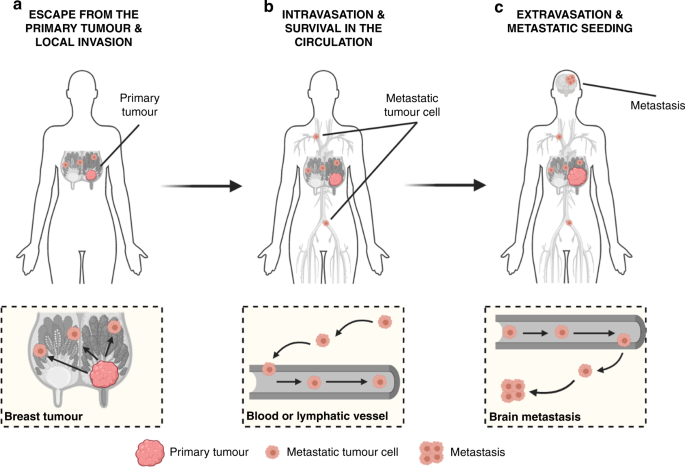
\includegraphics[width=0.8\textwidth]{../figs/introduction/process_of_metastatic_breast_cancer.png}}
        \caption{Process of Metastatic Breast Cancer \cite{RefWorks:RefID:364-riggio2020lingering}.}
        \label{fig:introduction:process_of_metastatic_breast_cancer}
\end{figure}

\subsection{Treatment of Breast Cancer\label{sec:introduction:treatmentofbreastcancer}}

\subsubsection{Stages of Breast Cancer\label{sec:introduction:breastcancer:stagesofbreastcancer}}
% Early vs late stage
Breast cancer is classified in stages ranging from 0 to IV based on the cancer's characteristics such as tumor size~\cite{RefWorks:RefID:151-2025breast}.

Stage 0 breast cancer is described as non-invasive, meaning the cancer cells are confined to the ducts or lobules in the breast and have not spread to surrounding healthy tissue~\cite{RefWorks:RefID:151-2025breast}.

Stage I breast cancer is invasive, meaning the cancer cells have spread to surrounding healthy tissue. In stage I breast cancer, the tumor is up to 2cm in size but invading cancer cells are no more than 1mm. Stage I is classified as either IA or IB depending on the sevarity of the cancer.~\cite{RefWorks:RefID:151-2025breast}.

Stage II breast cancer is used when the cancer is larger than 2cm but no larger than 5cm, or if the cancer has spread to one to three nearby lymph nodes. Similar to stage I breast cancer, stage II breast cancer can be subdivided into IIA and IIB~\cite{RefWorks:RefID:151-2025breast}.

Stage II breast cancer can be divided into IIIA, IIIB, and IIIC. This stage describes invasive breast cancer that is larger than 5cm or is found in four to nine nearby lymph nodes (IIIA), has spread to the chest wall or skin of the breast (IIIB), or has spread to ten or more nearby lymph nodes or to lymph nodes above or below the collarbone (IIIC)~\cite{RefWorks:RefID:151-2025breast}.

Lastly, stage IV breast cancer describes cancer that has metastasized, or spread, to other parts of the body such as the lungs, liver, bones, or brain~\cite{RefWorks:RefID:151-2025breast}.

Breast cancer stages can be divided into early and late stage breast cancer. Early-stage breast cancer incudes stages 0, I, and IIA while late-stage breast cancer includes stages IIB, III, and IV~\cite{RefWorks:RefID:365-stages}. Table~\ref{tab:introduction:breastcancer:stages} summarizes the stages of breast cancer.

\begin{table}[h!]
        \centering
        \begin{tabular}{|c|c|c|}
                \hline
                \textbf{Stage} & \textbf{Description}                                       & \textbf{Early/Late Stage} \\
                \hline
                0              & Non-invasive, confined to ducts or lobules                 & Early                     \\
                \hline
                I              & Invasive, tumor up to 2cm, invading cells no more than 1mm & Early                     \\
                \hline
                IIA            & Tumor 2-5cm or spread to 1-3 lymph nodes                   & Early                     \\
                \hline
                IIB            & Tumor larger than 5cm or spread to 1-3 lymph nodes         & Late                      \\
                \hline
                IIIA           & Tumor larger than 5cm or found in 4-9 lymph nodes          & Late                      \\
                \hline
                IIIB           & Spread to chest wall or skin of breast                     & Late                      \\
                \hline
                IIIC           & Spread to 10+ lymph nodes or above/below collarbone        & Late                      \\
                \hline
                IV             & Metastasized to other parts of the body                    & Late                      \\
                \hline
        \end{tabular}
        \caption{Stages of Breast Cancer~\cite{RefWorks:RefID:151-2025breast, RefWorks:RefID:365-stages}.}
        \label{tab:introduction:breastcancer:stages}
\end{table}

\subsubsection{Current Treatment Options\label{sec:introduction:breastcancer:currenttreatmentoptions}}
% Lumpectomy vs mastectomy

\subsection{Motivation\label{sec:introduction:motivation}}
This is a subsection of the background in the introduction!
